\subsection{2-Connected Graphs and their Properties}
\begin{definition}
    A graph is 2-connected if it cannot be separated into two components by removing a single vertex
\end{definition}
\begin{center}
    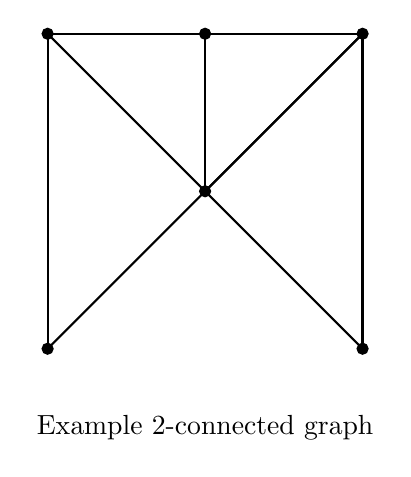
\begin{tikzpicture}
        \draw[black, thick] (0,0) -- (0,4);
        \draw[black, thick] (0,0) -- (4,4);
        \draw[black, thick] (4,0) -- (4,4);
        \draw[black, thick] (2,2) -- (4,4);
        \draw[black, thick] (2,2) -- (2,4);
        \draw[black, thick] (0,4) -- (4,4);
        \draw[black, thick] (0,4) -- (4,0);
        \foreach \x/\y in {0/0, 0/4, 2/2, 2/4, 4/0, 4/4} {
                \filldraw[black] (\x,\y) circle (2pt);
            }
        \node at (2,-1,0) {Example 2-connected graph};
    \end{tikzpicture}
    \hspace{2cm}
    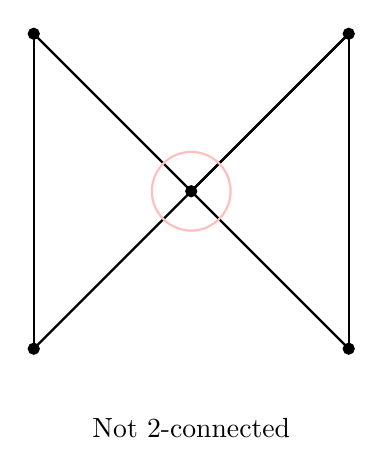
\begin{tikzpicture}
        \draw[black, thick] (0,0) -- (0,4);
        \draw[black, thick] (0,0) -- (4,4);
        \draw[black, thick] (4,0) -- (4,4);
        \draw[black, thick] (2,2) -- (4,4);
        \draw[black, thick] (0,4) -- (4,0);
        \draw[pink, thick] (2,2) circle (0.5);
        \foreach \x/\y in {0/0, 0/4, 2/2, 4/0, 4/4} {
                \filldraw[black] (\x,\y) circle (2pt);
            }
        \node at (2,-1,0) {Not 2-connected};
    \end{tikzpicture}
\end{center}
\begin{theorem}
    Mọi cặp đỉnh trong đồ thị 2-connected đều nằm trên cùng một chu trình.
    \begin{proof}
        Quy nạp:

        Trường hợp cơ bản: $u$ kề $v$
        \begin{center}
            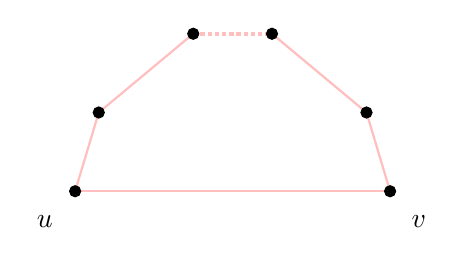
\begin{tikzpicture}
                \draw[pink, thick] (0,0) -- (0.3,1);
                \draw[pink, thick] (0.3,1) -- (1.5,2);
                \draw[densely dotted, pink, ultra thick] (1.5,2) -- (2.5,2);
                \draw[pink, thick] (2.5,2) -- (3.7,1);
                \draw[pink, thick] (3.7,1) -- (4,0);
                \draw[pink, thick] (0,0) -- (4,0);
                \node at (0,0,1) {$u$};
                \node at (4.75,0,1) {$v$};
                \filldraw[black] (0,0) circle (2pt);
                \filldraw[black] (0.3,1) circle (2pt);
                \filldraw[black] (1.5,2) circle (2pt);
                \filldraw[black] (2.5,2) circle (2pt);
                \filldraw[black] (3.7,1) circle (2pt);
                \filldraw[black] (4,0) circle (2pt);
            \end{tikzpicture}
        \end{center}
        Quy nạp: $u,v$ có khoảng cách $d+1$
        \begin{center}
            \begin{tikzpicture}
                \draw[pink, thick] (0,0) -- (0.3,1);
                \draw[pink, thick] (0.3,1) -- (1.5,2);
                \draw[densely dotted, pink, ultra thick] (1.5,2) -- (2.5,2);
                \draw[pink, thick] (2.5,2) -- (3.7,1);
                \draw[pink, thick] (3.7,1) -- (4,0);
                \draw[pink, thick] (0,0) -- (2,0);
                \draw[black, thick] (3,0) -- (4,0);
                \draw[pink, thick] (4,0) -- (5,0);
                \draw[densely dotted, black, ultra thick] (2,0) -- (3,0);
                \draw[pink, thick] (2.5,0) -- (3.25,-1);
                \draw[pink, thick] (3.35,-1) -- (4.5,-1);
                \draw[pink, thick] (5,0) -- (4.5,-1);
                \draw[pink, thick] (2,0) -- (2.5,0);

                \node at (0,0,1) {$u$};
                \node at (5.75,0,1) {$v$};
                \node at (4.4,0,1) {$w$};
                \filldraw[black] (0,0) circle (2pt);
                \filldraw[black] (0.3,1) circle (2pt);
                \filldraw[black] (1.5,2) circle (2pt);
                \filldraw[black] (2.5,2) circle (2pt);
                \filldraw[black] (3.7,1) circle (2pt);
                \filldraw[black] (1,0) circle (2pt);
                \filldraw[black] (2,0) circle (2pt);
                \filldraw[black] (3,0) circle (2pt);
                \filldraw[black] (4,0) circle (2pt);
                \filldraw[black] (5,0) circle (2pt);
                \filldraw[black] (3.25,-1) circle (2pt);
                \filldraw[black] (4.5,-1) circle (2pt);

                \draw [decorate, decoration = {calligraphic brace, mirror, raise=5pt}] (0,-1.5) --  (4,-1.5) node[pos=0.5,below=10pt,black]{$d$};
            \end{tikzpicture}
        \end{center}
    \end{proof}
\end{theorem}